\documentclass[9pt, a4paper, oneside]{amsart}

\usepackage[final]{pdfpages}

\usepackage{enumitem}
\usepackage{parskip}
\usepackage{fancyhdr}
\usepackage{color}
\usepackage{multicol}
\pagestyle{fancy}

\newlist{questions}{enumerate}{1}
\setlist[questions, 1]{label = \bf Q.\arabic*., itemsep=1em}

\lhead{\scshape Apurva Nakade}
\rhead{\scshape Honors Single Variable Calculus}
\renewcommand*{\thepage}{\small\arabic{page}}
\title{Problem Set 05}

\begin{document}

\maketitle
\thispagestyle{fancy}


\section*{Part 1 - Differentiation}
\begin{questions}
	\item Do \textbf{Q.1} (parts (i) - (viii)) and \textbf{Q.3} from Chapter 10 of the book.

	\item If $ f$ is three times differentiable and $ f'(x) \neq 0$ the \textbf{Schwarzian derivative} of $ f$ at $ x$ is defined to be
	\begin{align*}
		\frak{D}f(x) & = \dfrac{f'''(x)}{f'(x)} - \dfrac{3}{2} \left(\dfrac{f''(x)}{f'(x)}\right)^2
	\end{align*}
	Show that $ \frak{D}g=0$ for the function $ g(x) = \dfrac{ax + b}{cx + d}$ with $ ad - bc \neq 0$.

	\item
	\begin{enumerate}
		\item A number $ a$ is called a \textbf{double root} of a polynomial $ f$ if $ f(x) = (x-a)^2 g(x)$ for some polynomial $ g$. Prove that $ a$ is a double root of $ f$ if and only if both $ f$ and $ f'$ vanish at $ a$.
		\item When does $ f(x) = ax^2 + bx + c$ have a double root? What does the condition say geometrically?
	\end{enumerate}


	\item
	\begin{enumerate}\item Try to prove the following formulae using the definition of derivative\footnote{You can use the following trigonometric identities
			\begin{align*}
				\sin(a + b) & = \sin a \cos b + \sin b \cos a \\
				\cos(a + b) & = \cos a \cos b - \sin a \sin b
			\end{align*}}
		\begin{align*}
			(\sin x)' = \cos x &   & (\cos x)' = -\sin x
		\end{align*}
		What identities \emph{should be true} (in terms of limits $ \lim \limits_{h \rightarrow 0}$) for the above formulae to hold?
		\item Look at the graphs of $ \sin x$ and $ \cos x$ near $ x=0$, and come up with a {heuristic argument} as to why these identities might true.
	\end{enumerate}
\end{questions}










\newpage
\section*{Part 2 - Inverse Functions}
\begin{questions}[resume]
	\item For this problem assume that $ x \neq 0$.
	\begin{enumerate}
		\item Using induction and product rule show that $ (x^n)' = n x^{n-1}$ when $ n$ is a non-negative integer.
		\item Using the quotient rule show that $ (x^n)' = n x^{n-1}$ when $ n$ is a negative integer.
		\item Using the fact that $ x^{1/n}$ is the inverse of $ x^n$ show that $ (x^n)' = n x^{n-1}$ when $ n = 1/m$ for some non-zero integer $ m$.
		\item Using chain rule show that $ (x^n)' = n x^{n-1}$ when $ n$ is a rational number.
		\item Can you think of some way of extending this to the case when $ n$ is an irrational number?
	\end{enumerate}

	\item Determine the derivatives of $ \sin^{-1}x$ and $ \tan^{-1}x$. (Later on we'll use these inverse functions to rigorously define $ \sin x$.)

	\item Suppose the functions $ f$ and $ g$ are increasing everywhere i.e. $ f(x) > f(y)$ and $ g(x) > g(y)$ for all $ x > y$.
	\begin{enumerate}
		\item Which of the functions $ f+g$, $ f.g$ and $ f \circ g$ are necessarily increasing.
		\item Show that $ f^{-1}$ is also an increasing function.
		\item Determine $ (f \circ g)^{-1}$ in terms of $ f^{-1}$ and $ g^{-1}$.
		\item Find $ g^{-1}$ in terms of $ f^{-1}$ if $ g(x) = 1+ f(x)$.
	\end{enumerate}

\end{questions}


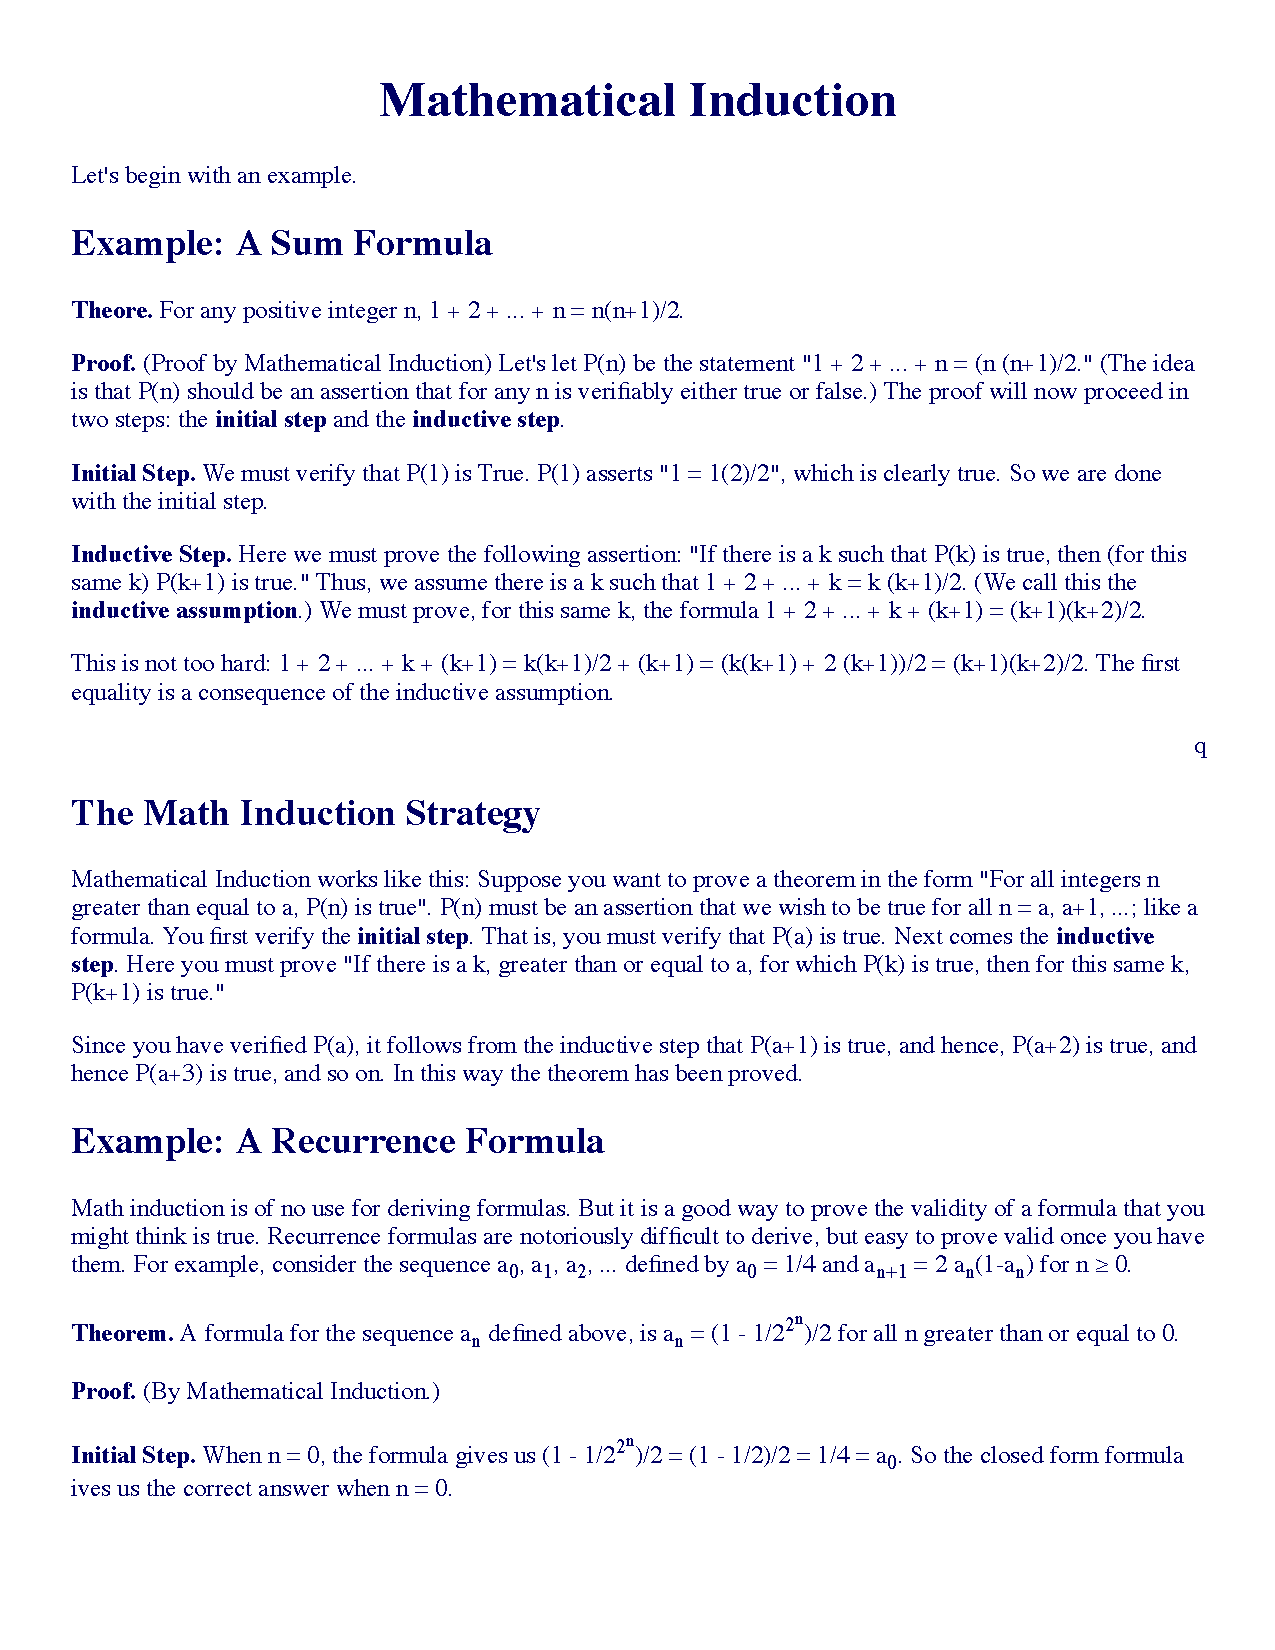
\includepdf[pages=-]{Mathematical_Induction.pdf}







\end{document}
